\documentclass[11pt]{article}

\usepackage{minted,xcolor}
\usemintedstyle{monokai}
\definecolor{bg}{HTML}{282828}
\usepackage{xcolor, colortbl}
\usepackage{graphicx}
\usepackage{titlesec}
\usepackage[hmargin=2cm,vmargin=2.5cm]{geometry}
\usepackage{fancyhdr}
\usepackage{hyperref}
\usepackage{caption}
\usepackage{subcaption}

\definecolor{tableaublue}{RGB}{78, 121, 167}

\hypersetup{
    colorlinks=true,
    linkcolor=black,
    filecolor=tableaublue,      
    urlcolor=tableaublue,
    pdftitle={Overleaf Example},
    pdfpagemode=FullScreen,
}

\setlength\parindent{0cm}
\setlength\headheight{28pt}

\titleformat{\section}{\normalfont\Large\bfseries}{Part~\thesection:}{6pt}{}[{\titlerule[0.5pt]}]
\titleformat{\subsection}{\normalfont\large\bfseries}{Exercise~\thesubsection:}{6pt}{}

\graphicspath{ {./img/} }

% \title{Practical’s instruction – Networks (week 7)}
% \author{CSC3833 - Data Visualization and Visual Analytic}

\begin{document}

\pagestyle{fancy}
\renewcommand{\headrulewidth}{0pt}
\fancyhead[L]{CSC8626/CSC8642 - Data Visualization}
\fancyhead[R]{2023 / 2024}

\begin{center}
\vspace*{1cm}
{\textbf {\Huge Practical 2}}\\
\vspace*{0.5cm}
{\textbf {\huge Introduction to Power BI}}
\vspace*{1cm}
\end{center}

\section{Creative Industries}

Part one of this assessment will guide you thought loading, filtering, and displaying creative industries data of the North East using Power BI.\\

In 2001 the Creative Industries were defined by the Department for Digital, Culture, Media and Sport (DCMS) as those industries "which have their origin in individual creativity, skill and talent and which have a potential for wealth and job creation through the generation and exploitation of intellectual property" (see \href{https://www.gov.uk/government/publications/dcms-sectors-economic-estimates-methodology}{UK Government 2021}).\\

Currently DCMS uses a measurement that builds on this original definition but is based on the ‘creative intensity’ of an industry. A subsector (like Publishing or Architecture) is normally deemed creative when more than thirty percent of its workforce are doing what we call ‘creative occupations’ (e.g. they might be designers, producers or games developers). To be part of the Creative Industries, sectors also have to meet other threshold criteria (see \href{https://assets.publishing.service.gov.uk/government/uploads/system/uploads/attachment_data/file/499683/CIEE_Methodology.pdf}{DCMS 2016}).\\

The resulting definition of the Creative Industries comprises the following nine subsectors:

\begin{itemize}
    \itemsep0em 
    \item  Advertising and marketing
    \item  Architecture
    \item  Crafts
    \item  Design and designer fashion
    \item  Film, TV, video, radio and photography
    \item  IT, software and computer services
    \item  Publishing
    \item  Museums, Galleries and Libraries
    \item  Music, performing and visual arts
\end{itemize}

Source: \href{https://pec.ac.uk/news/national-statistics-on-the-creative-industries}{National Statistics on the Creative Industries}

\subsection*{Data}

\underline{File name}: CreativityData\_NorthEast.xls\\
This file is available on the Canvas page of the module, which can be accessed at \href{https://ncl.instructure.com/courses/49730}{link}.\\

\underline{Parameters}:
\begin{table}[h!]
    \centering
    \begin{tabular}{|l|m{8cm}|}
        \hline
        TTWA & Travel To Work Area: area where the population would commute to a larger town for the purposes of employment \\
        \hline
        region & region of England \\
        \hline
        creative\_cluster & Boolean indicating whether the area is or not a creative cluster \\
        \hline
        Number of creative businesses &  \\
        \hline
        Creative Businesses (\% of total) &  \\
        \hline
        Creative employment &  \\
        \hline
        Creative employment (\% of total) &  \\
        \hline
        Creative jobs &  \\
        \hline
        Creative jobs (\% of total) &  \\
        \hline
        Sales per worker (£GBP) &  \\
        \hline
        Average firm size &  \\
        \hline
        Creative GVA (£GBP) &  \\
        \hline
        Creative GVA (\% of total) &  \\
        \hline
        $<$\textit{dateRange}$>$\_$<$\textit{industrialSector}$>$\_business.count & number of business per sector for a specific date range (2007/2010 or 2011/2014)  \\
        \hline
        $<$\textit{dateRange}$>$\_$<$\textit{industrialSector}$>$\_turnover & turnover per sector for a specific date range \\
        \hline
        $<$\textit{dateRange}$>$\_$<$\textit{industrialSector}$>$\_employment & employment per sector for a specific date range \\
        \hline
        $<$\textit{dateRange}$>$\_$<$\textit{industrialSector}$>$\_turn\_pw &  \\
        \hline
        $<$\textit{dateRange}$>$\_$<$\textit{industrialSector}$>$\_work\_pb &  \\
        \hline
        Qualifiers\_compsci\_2014 &  \\
        \hline
        Qualifiers\_art.design\_2014 &  \\
        \hline
        FTE\_Researchers\_arts and design\_2013 &  \\
        \hline
        FTE\_Researchers\_computer science\_2013 &  \\
        \hline
        HE\_BCI\_business.turnover\_TH\_GBP\_2014 &  \\
        \hline
        HE\_BCI\_sme.engagement\_TH\_GBP\_2014 &  \\
        \hline
        HE\_BCI\_sme.training\_TH\_GBP\_2014 &  \\
        \hline
        HE\_BCI\_event.attendees\_2014 &  \\
        \hline
    \end{tabular}
    \caption{Parameters contained within the dataset}
    \label{tab:my_label}
\end{table}

\subsection{Loading Data}

Open Power BI and click on the 'Get data' menu to load the creativity dataset.\\
\\
\\
\\
\\
\\
\\
\\
\\
\\
\\

\begin{figure}[h!]
    \centering
    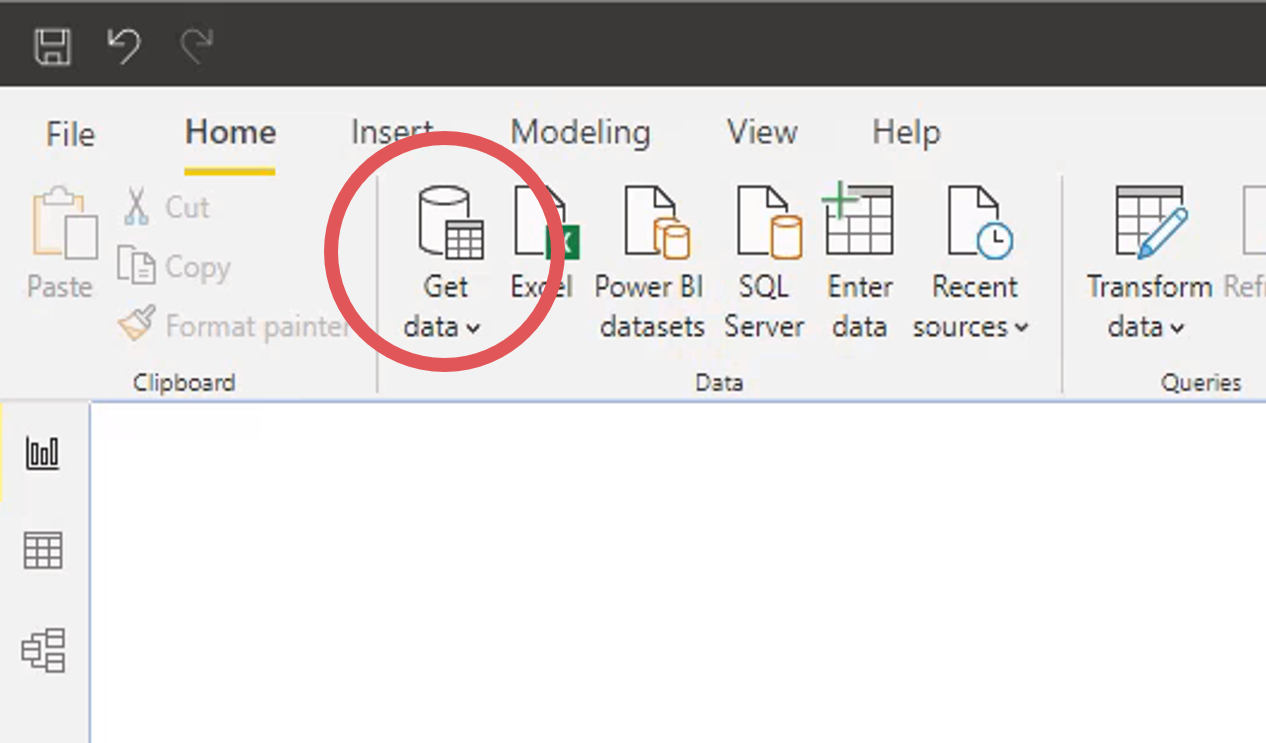
\includegraphics[width=.6\linewidth]{img/getData.png}
    % \caption{Caption}
    % \label{fig:enter-label}
\end{figure}

Select 'Sheet 1' and click load.

\begin{figure}[h!]
    \centering
    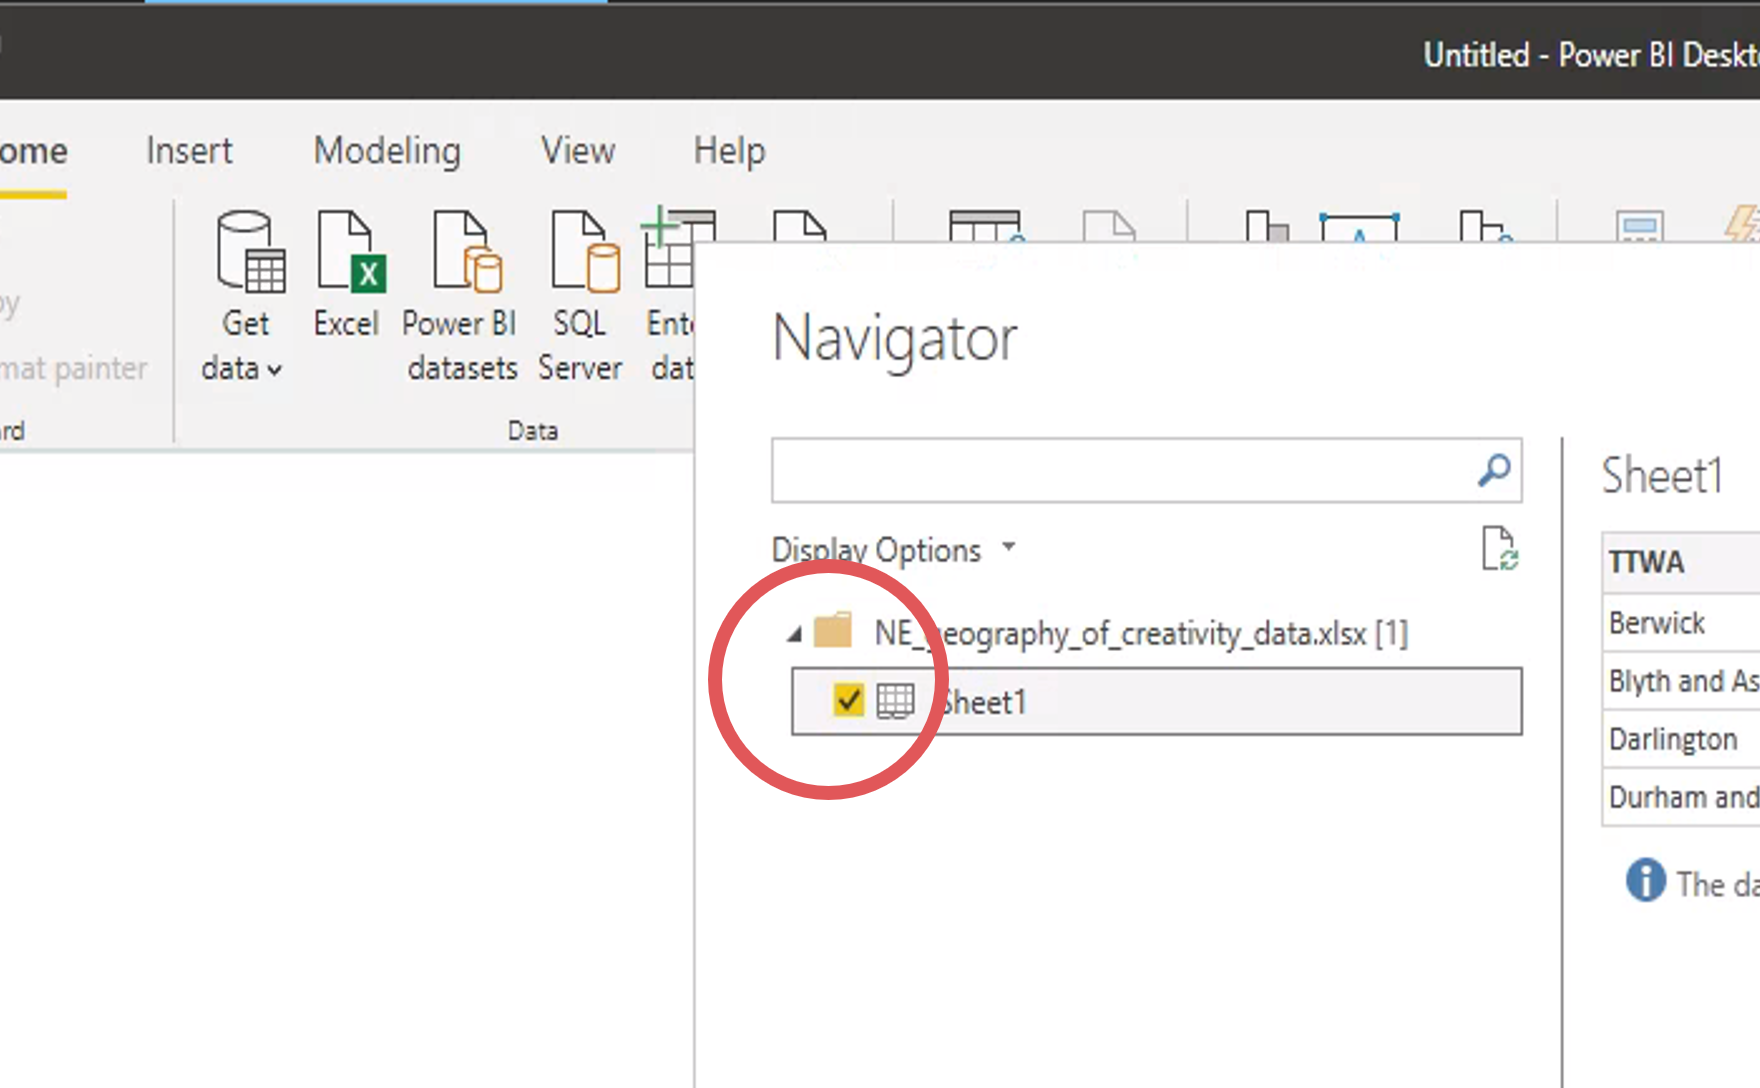
\includegraphics[width=.6\linewidth]{img/selectSheet.png}
    % \caption{Caption}
    % \label{fig:enter-label}
\end{figure}

Note that every column in the spreadsheet appears on the right panel.

\begin{figure}[h!]
    \centering
    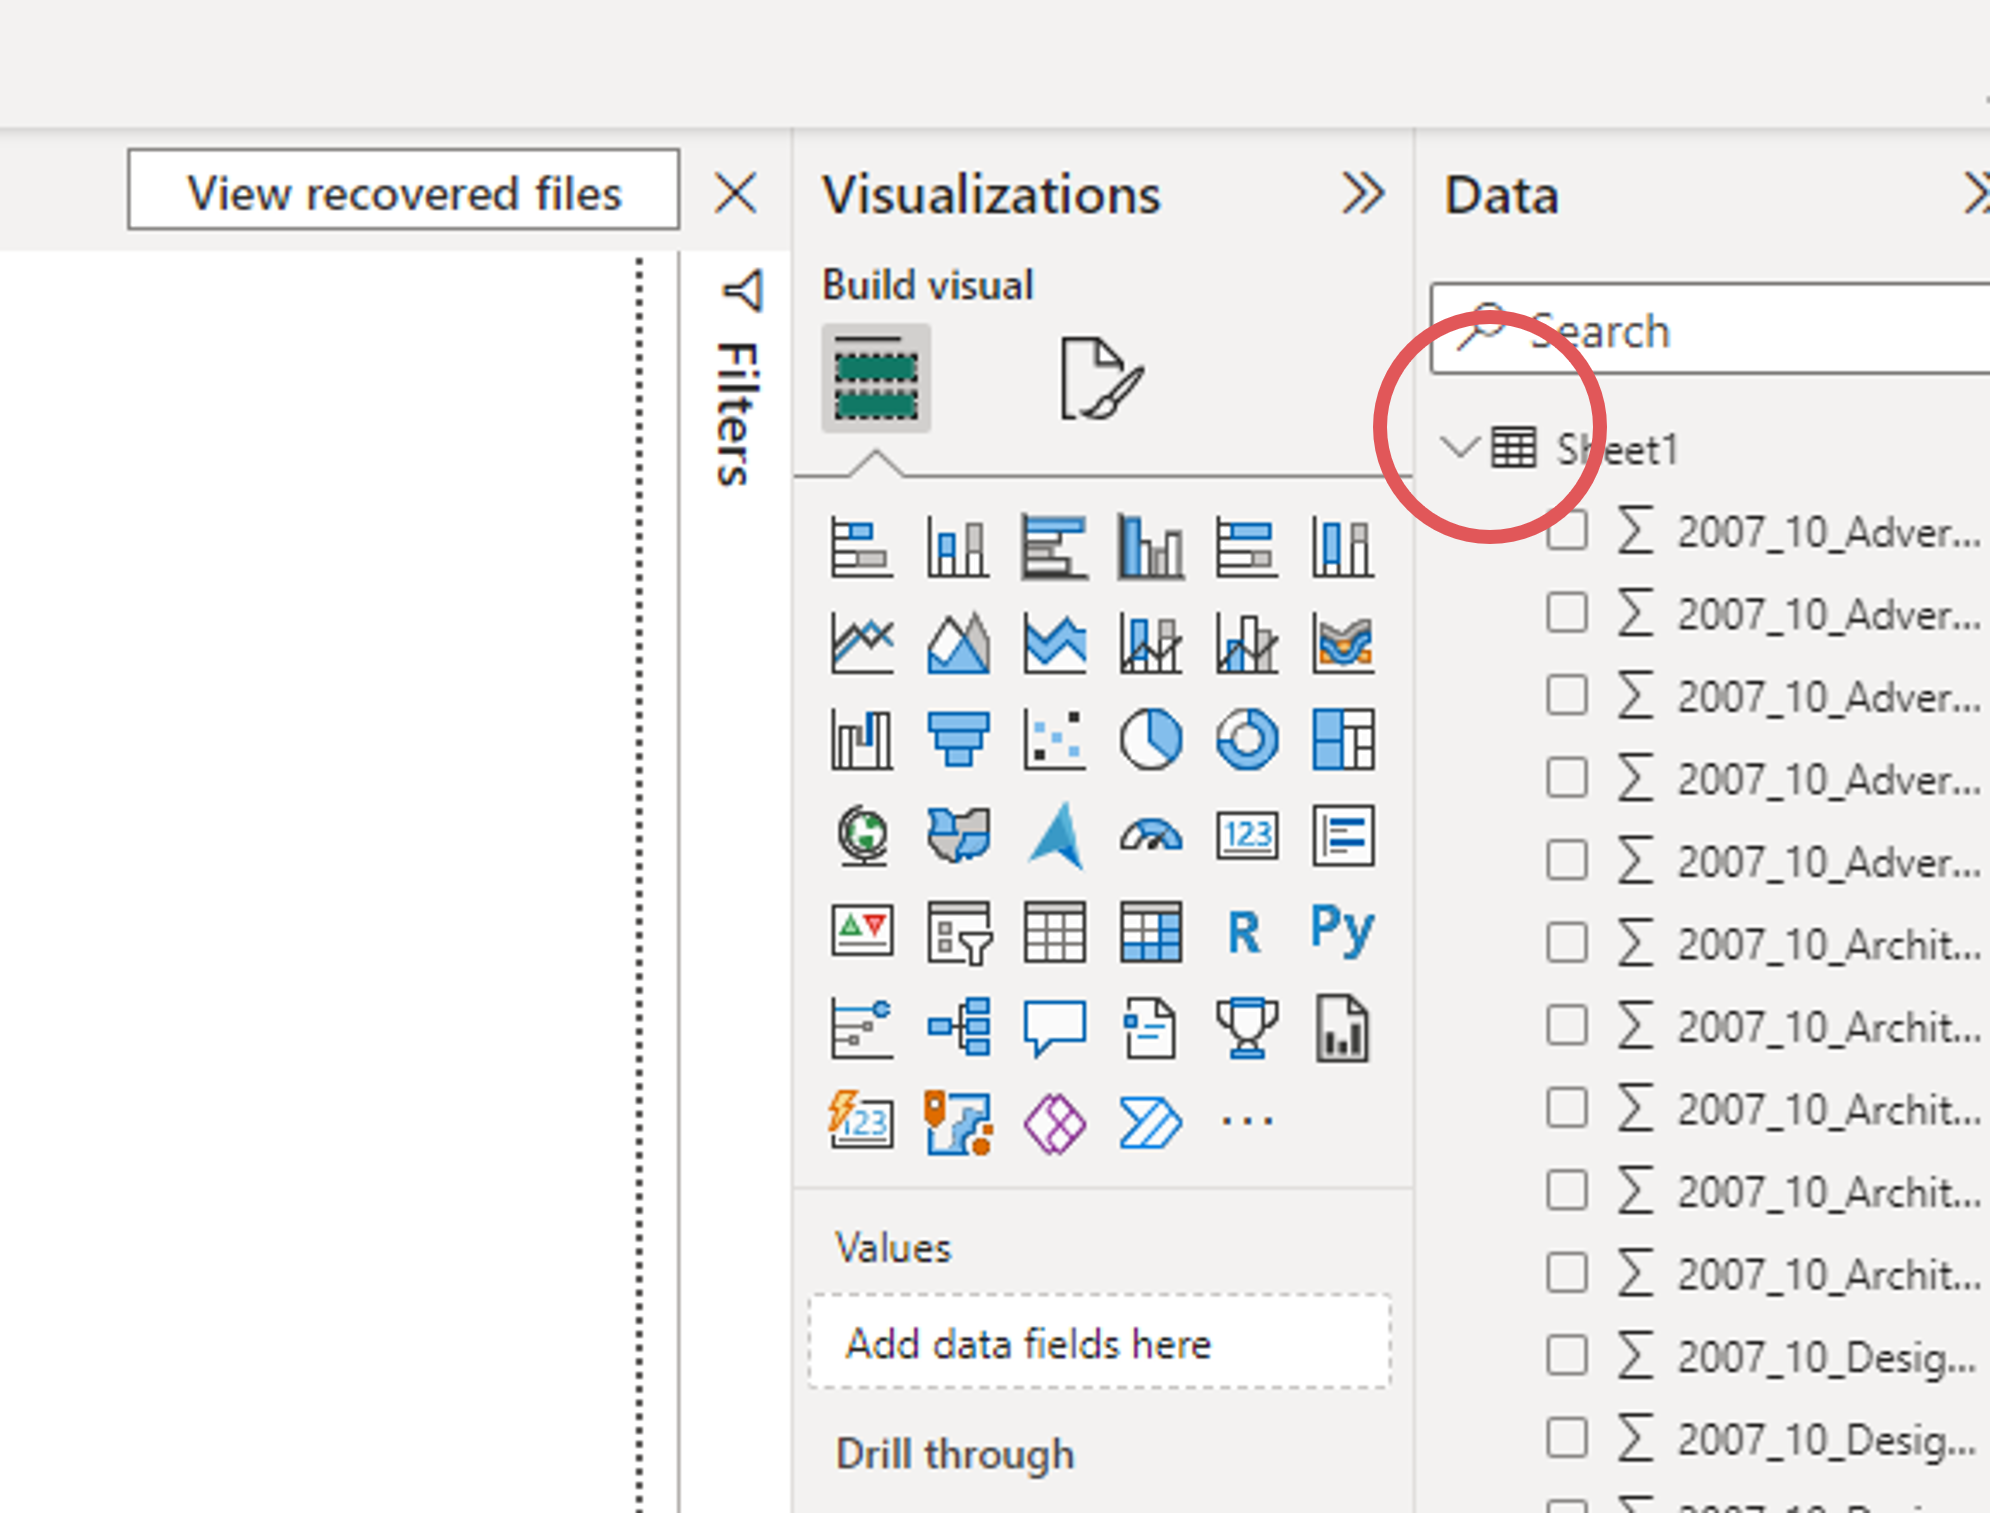
\includegraphics[width=.5\linewidth]{img/loadedData.png}
    % \caption{Caption}
    % \label{fig:enter-label}
\end{figure}

\clearpage

\subsection{Removing film sectors}

Click on 'Transform data' to shape the data.

\begin{figure}[h!]
    \centering
    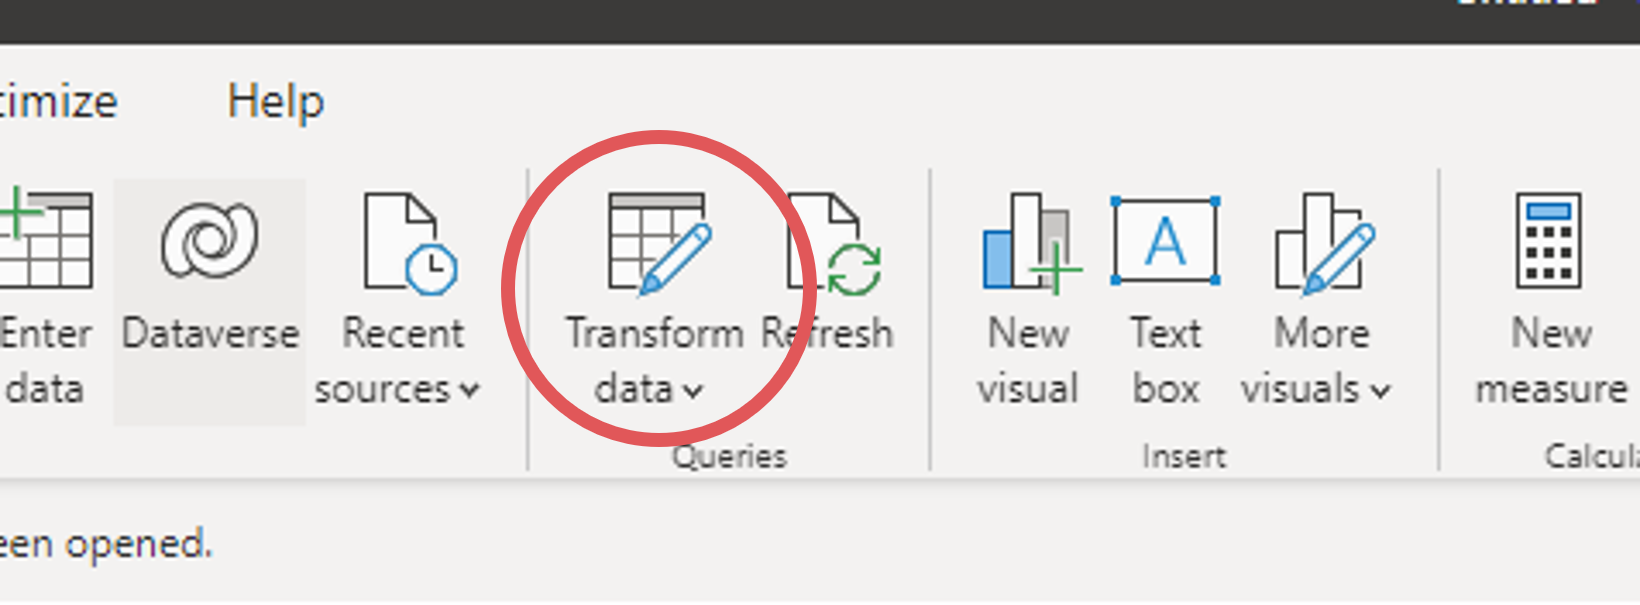
\includegraphics[width=.4\linewidth]{img/transformData.png}
    % \caption{Caption}
    % \label{fig:enter-label}
\end{figure}

Click on the 'Choose Columns' menu and unselect the ten columns specific to 'Film'.

\begin{figure}[h!]
    \centering
    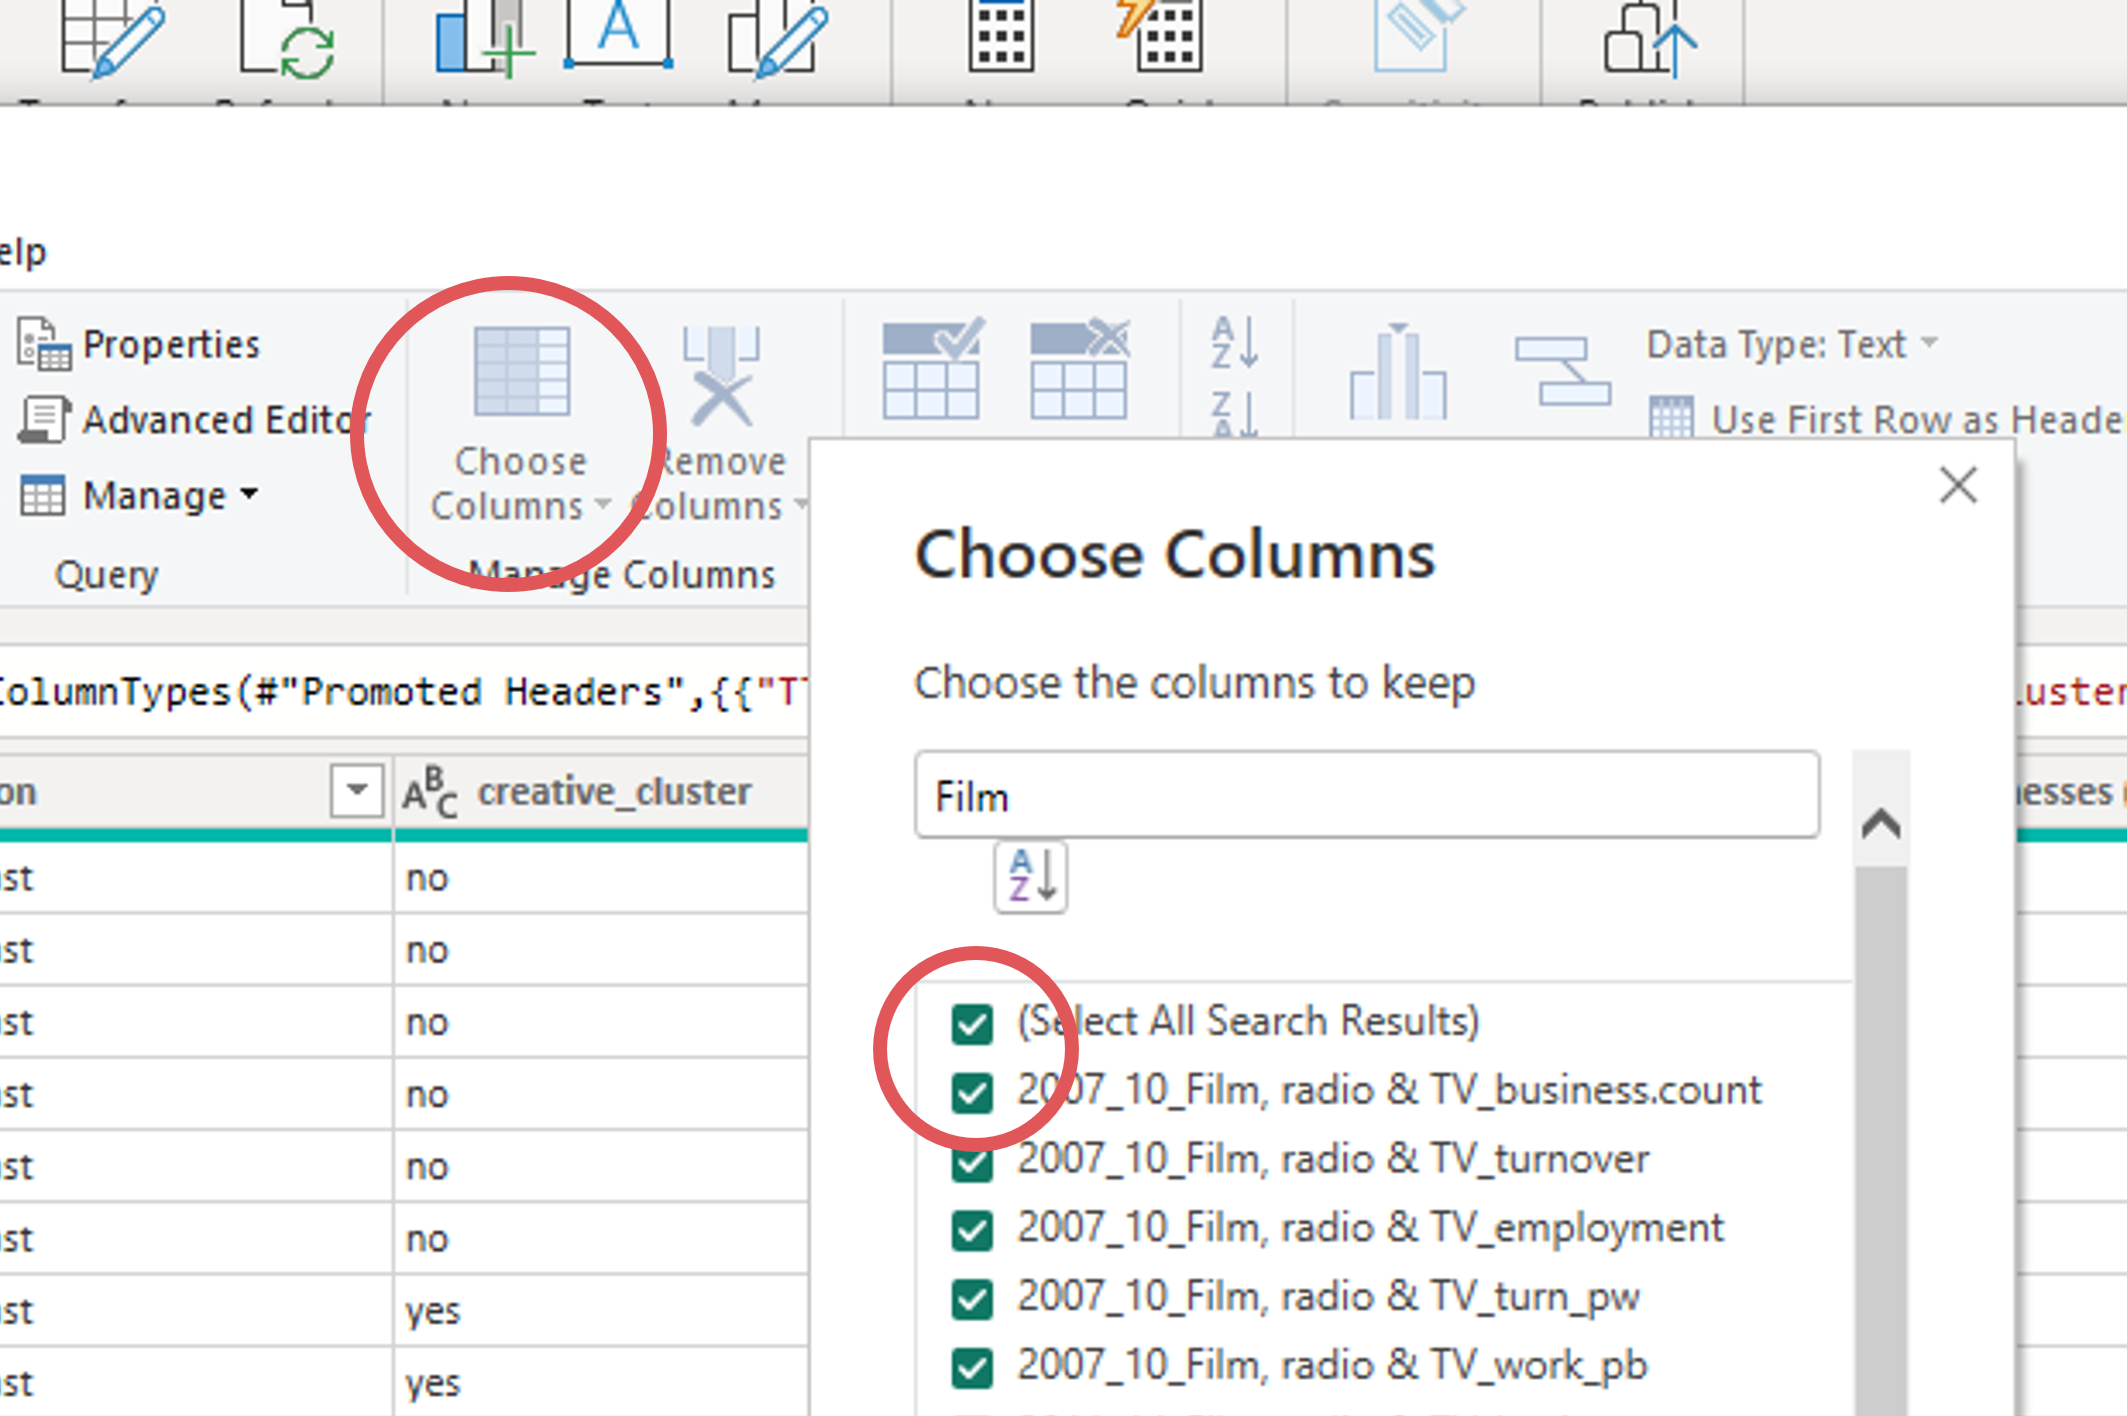
\includegraphics[width=.6\linewidth]{img/chooseColumn.png}
    % \caption{Caption}
    % \label{fig:enter-label}
\end{figure}

Click 'OK' then click 'Close and Apply' to apply the filters to the data.

\begin{figure}[h!]
    \centering
    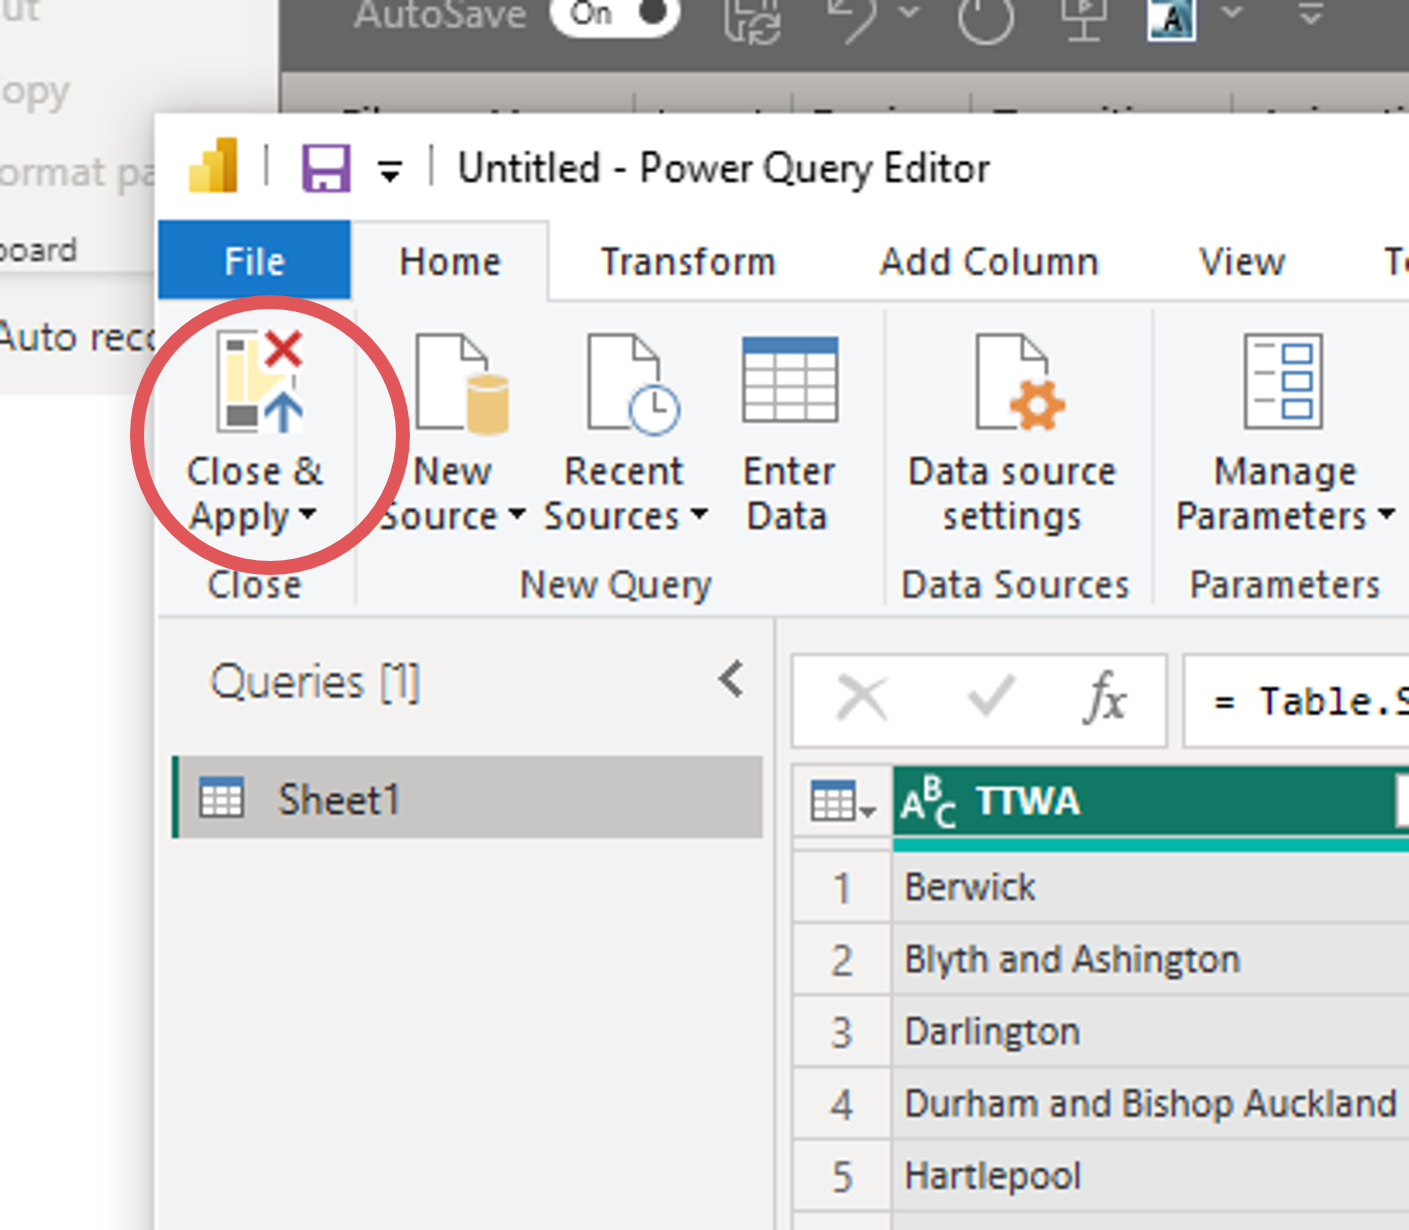
\includegraphics[width=.5\linewidth]{img/applyTransform.png}
    % \caption{Caption}
    % \label{fig:enter-label}
\end{figure}

Now the active fields only show those we decided to keep. NB you can go always back and edit the queries.

\subsection{Display creative business count per area}

Click on the icon for 'Clustered column chart' in the 'Visualizations' panel and select or drag 'TTWA' and '2007\_All creative industries\_business.count' in the X and Y axis slots.

\begin{figure}[h!]
    \centering
    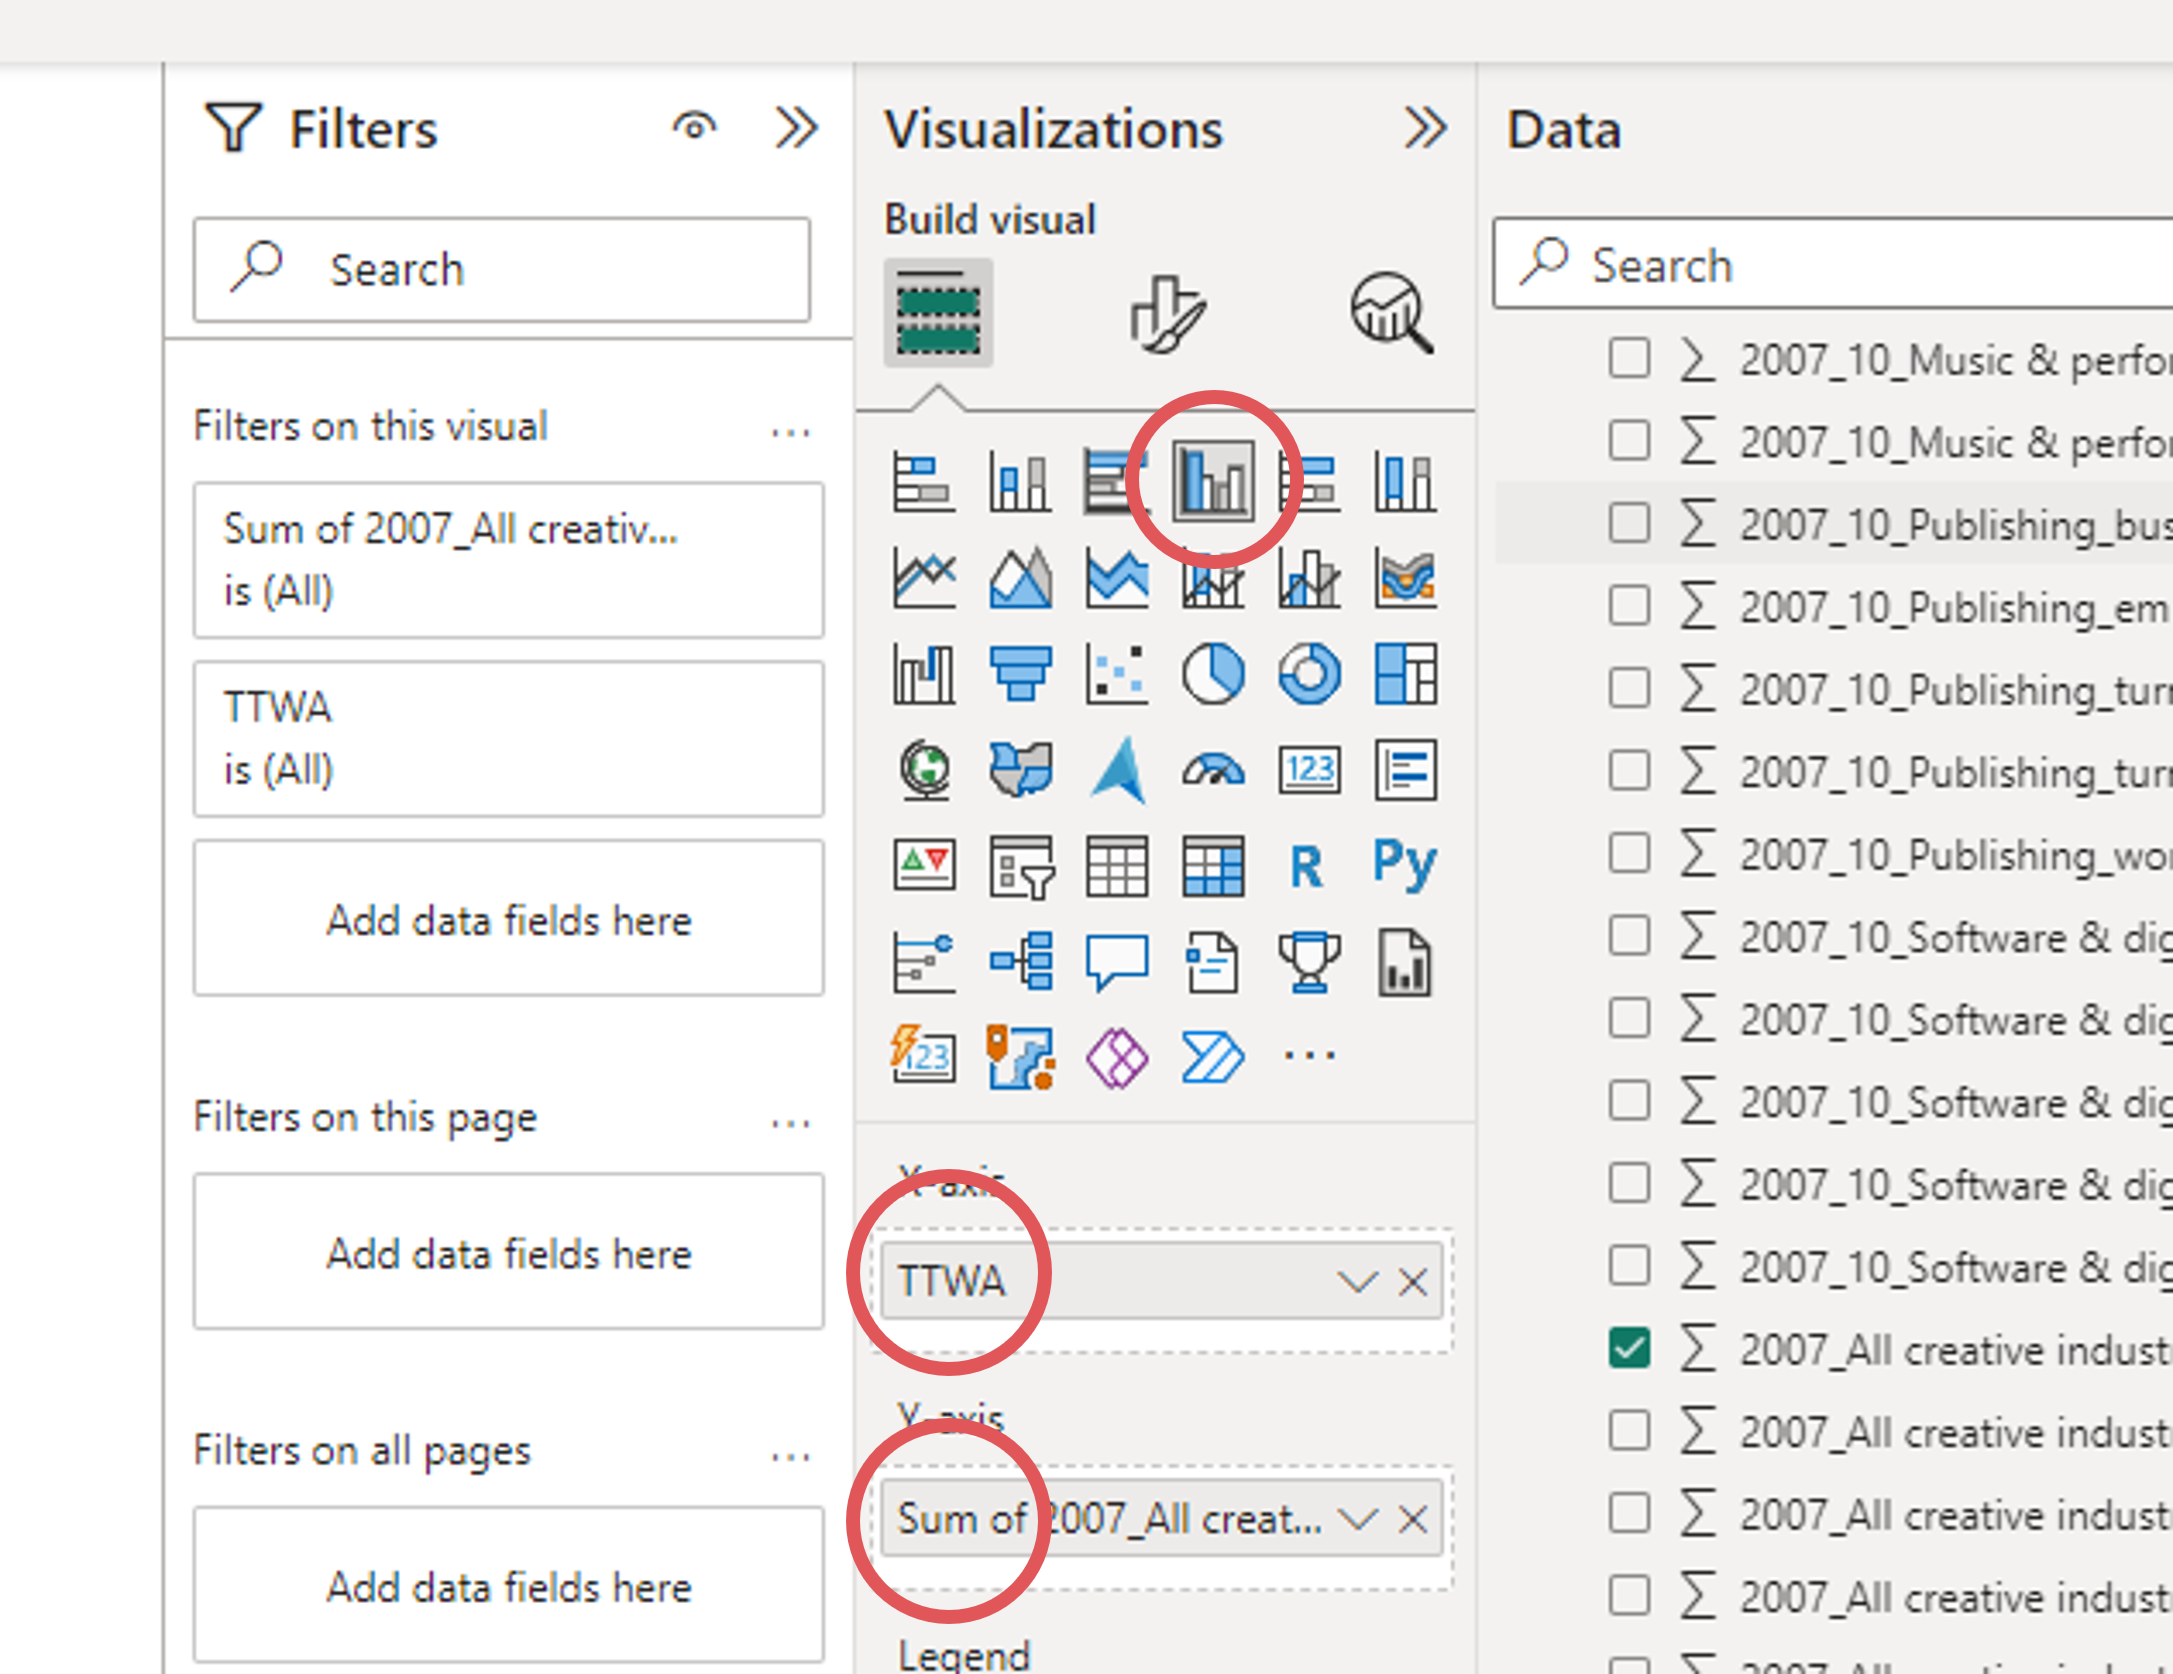
\includegraphics[width=.5\linewidth]{img/createCreativeChart.png}
    % \caption{Caption}
    % \label{fig:enter-label}
\end{figure}

You should get a similar result than the chart below.

\begin{figure}[h!]
    \centering
    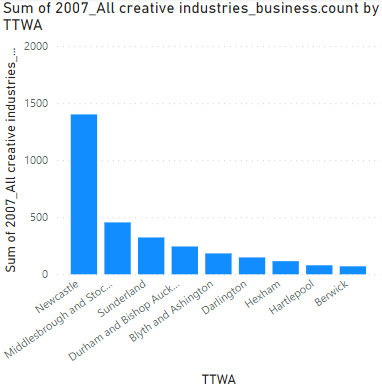
\includegraphics[width=.5\linewidth]{img/firstChart.png}
    % \caption{Expected result for exercise 1.3}
    % \label{fig:enter-label}
\end{figure}

\subsection{Customize your chart}

Click on the chart, then select 'Format you visual' on the 'Visualizations' panel. Click on 'General', then 'Title', and update the title of your chart to something more meaningful (e.g. Creative business count per area).\\

\begin{figure}[h!]
    \centering
    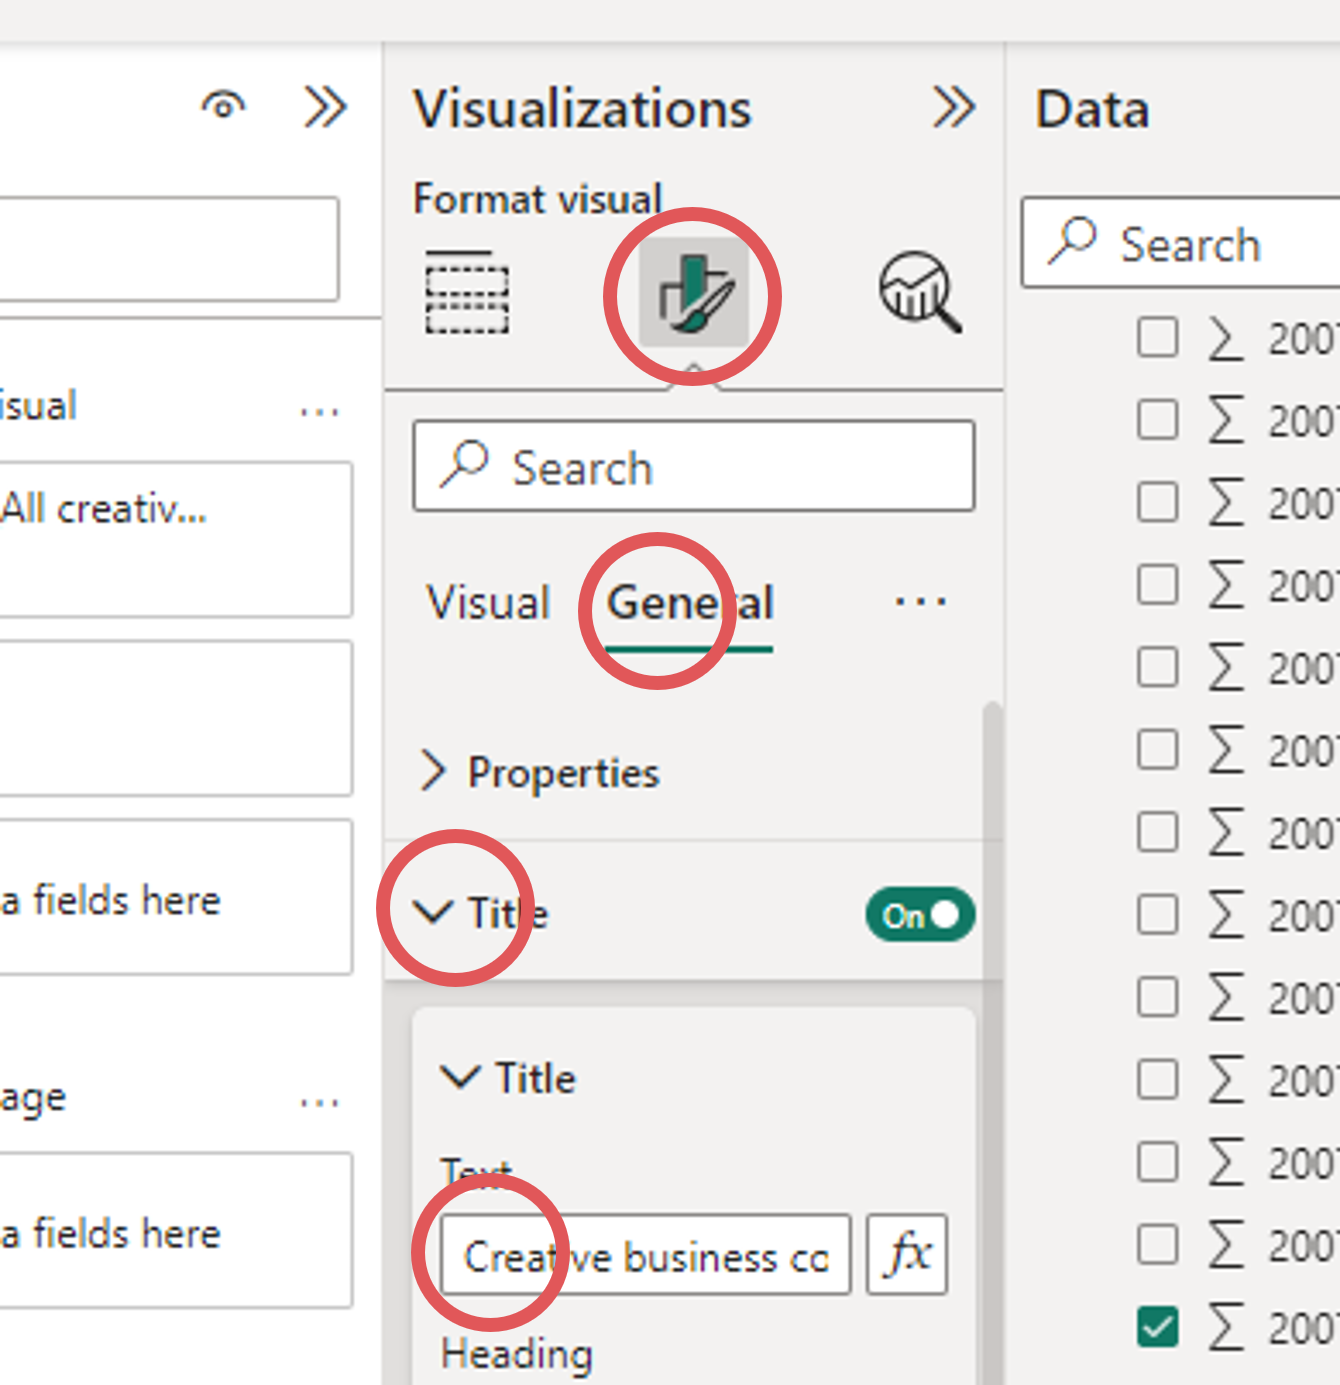
\includegraphics[width=.5\linewidth]{img/customizeChart.png}
    % \caption{Caption}
    % \label{fig:customizeChart}
\end{figure}

Click on 'Visual' $>$ 'Y-Axis' $>$ 'Title' and update the title text label to 'Creative business count'.\\
\\

\begin{figure}[h!]
    \centering
    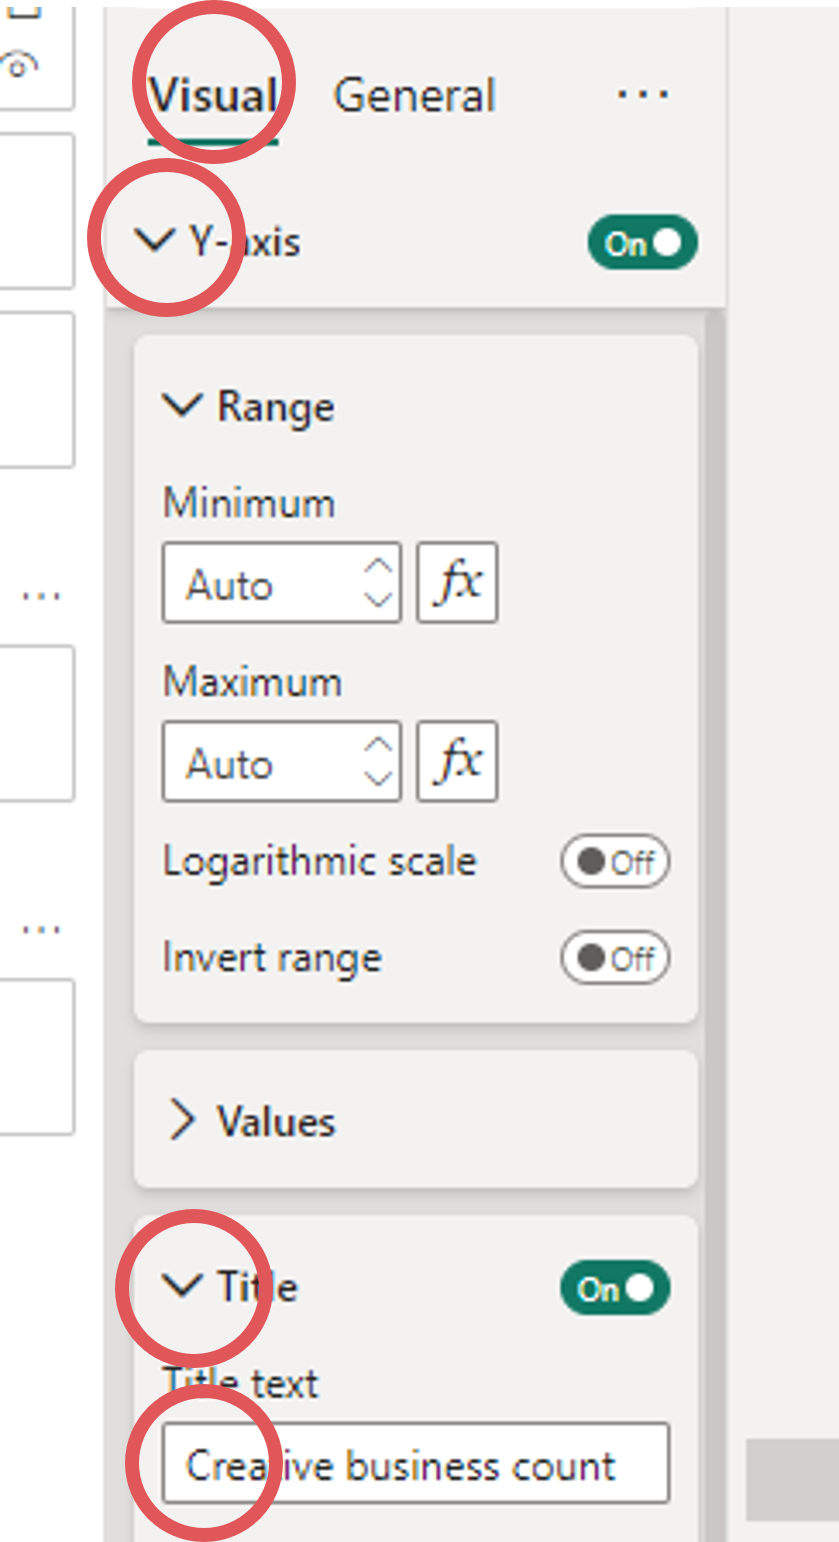
\includegraphics[width=.3\linewidth]{img/updateYaxisTitle.png}
    % \caption{Caption}
    % \label{fig:enter-label}
\end{figure}

Finally, change the colour of the bars in 'Visual' $>$ 'Columns' $>$ 'Colors' with one of the Tableau10 colours below.

\begin{figure}[h!]
    \centering
    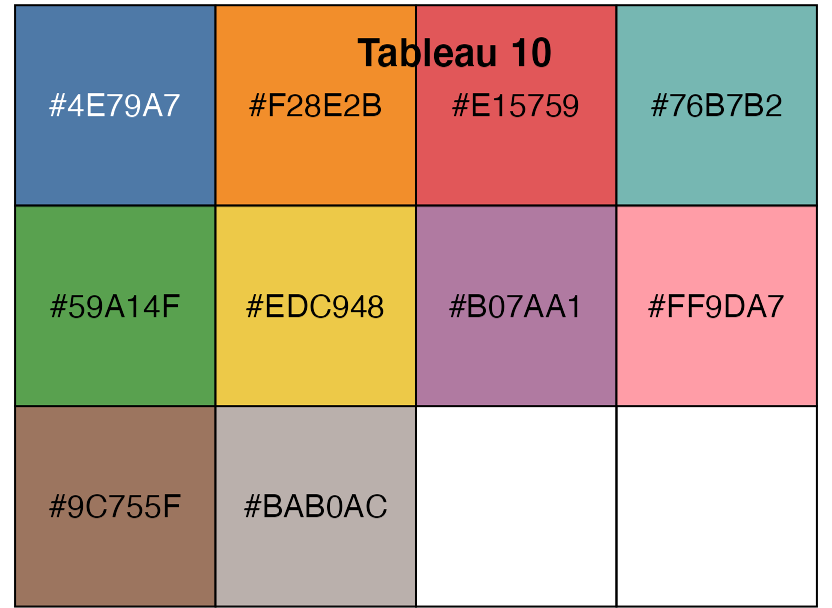
\includegraphics[width=.35\linewidth]{img/tableau10.png}
    % \caption{Set of 10 colours for Tableau software}
    % \label{fig:enter-label}
\end{figure}

You should get a  result similar to the chart below.\\

\begin{figure}[h!]
    \centering
    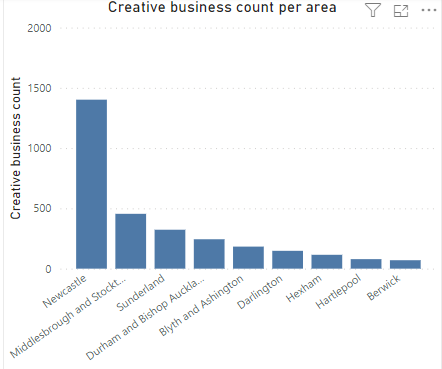
\includegraphics[width=.5\linewidth]{img/finalCreativeData.png}
    % \caption{Expected result for exercise 1.4}
    % \label{fig:enter-label}
\end{figure}

\clearpage

\section{North East Companies}

Part two involves the creation of a dashboard displaying North East companies data, which includes multiple bar charts.\\

Consider the nature of the data and determine the most suitable visual variables for representing them, such as color, size, position, and more. Additionally, ensure you customize the legend to offer clear and explicit visualizations.\\

To go further, read the Power BI tutorial which can be accessed at \href{https://learn.microsoft.com/en-us/power-bi/visuals/power-bi-visualization-customize-title-background-and-legend}{link}.

\subsection*{Data}

\underline{File}: CompanyData\_NorthEast.xls\\
This file is available on the Canvas page of the module, which can be accessed at \href{https://ncl.instructure.com/courses/49730}{link}.\\

\underline{Parameters}:

\begin{table}[h!]
    \centering
    \begin{tabular}{|l|m{8cm}|}
        \hline
        Company ID & company identifier \\
        \hline
        Turnover 2016 & company turnover (income or gross revenue) in 2016 \\
        \hline
        Turnover 2017 & company turnover (income or gross revenue) in 2017 \\
        \hline
        Percentage Growth & turnover growth percentage between 2016 and 2017 \\
        \hline
        Main SIC4 & sector identifier \\
        \hline
        Main SIC4 Name & sector name\\
        \hline
    \end{tabular}
    % \caption{Parameters contained within the dataset}
    % \label{tab:my_label}
\end{table}

\subsection{Company count per sector}

Display the company count per sector using a clustered column chart.\\

Creating a clustered column chart necessitates specifying an X-axis and a Y-axis parameter. The Y-axis values are aggregated based on the values of the X-axis and are presented in columns. The aggregation method, such as sum, average, or count, is often automatically selected.\\

To depict the count of companies per sector, select 'TTWA' as the X-axis and 'Company ID' as the Y-axis. Ensure that the 'Company ID' is aggregated using the 'count' function.\\

Take the time to customize your display.\\

\underline{Expected results}\\
\\
\\

\begin{figure}[h!]
    \centering
    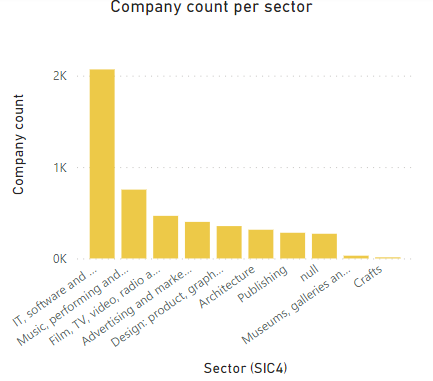
\includegraphics[width=.4\linewidth]{img/companyPerSector.png}
    % \caption{Expected result for the exercise 2.1}
    % \label{fig:companyPerSector}
\end{figure}

\subsection{Comparative income per sector between 2016 and 2017}

Within the same dashboard, display the total income per sector for the years 2016 and 2017 using a clustered column chart.\\

The clustered column chart is highly useful for comparing quantitative values as you can incorporate multiple Y-axis parameters. They will be automatically presented alongside each other, grouped by X-axis values.\\

For consistency, use similar names to the previous chart. Instead of modifying the X-axis title, you can directly rename the variable and use the variable label as the default title.\\

\underline{Expected results}

\begin{figure}[h!]
    \centering
    \begin{minipage}{.5\textwidth}
      \centering
      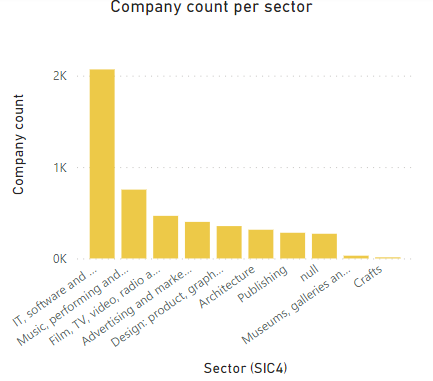
\includegraphics[width=.8\linewidth]{img/companyPerSector.png}
      % \captionof{figure}{Coloured cubes}
      % \label{fig:cubes}
    \end{minipage}%
    \begin{minipage}{.5\textwidth}
      \centering
      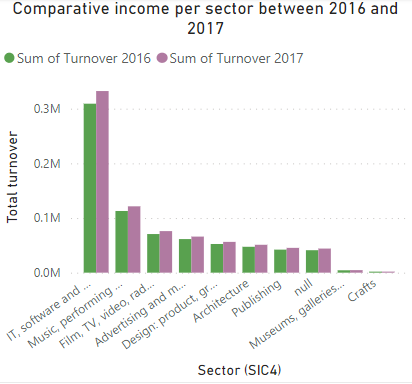
\includegraphics[width=.8\linewidth]{img/totalTurnover.png}
      % \captionof{figure}{Transparent sheets}
      % \label{fig:sheets}
    \end{minipage}
    % \caption{Expected result for the exercise 2.2}
    % \label{fig:totalTurnover}
\end{figure}

\subsection{Growth rate between 2016 and 2017}

Showcase the growth rate between 2016 and 2017.\\

Consider the most relevant way to display this information. Keep in mind that growth rates are typically presented as percentages, so summarizing them by sector may not be the most appropriate approach.\\

\underline{Expected results}

\begin{figure}[h!]
    \centering
    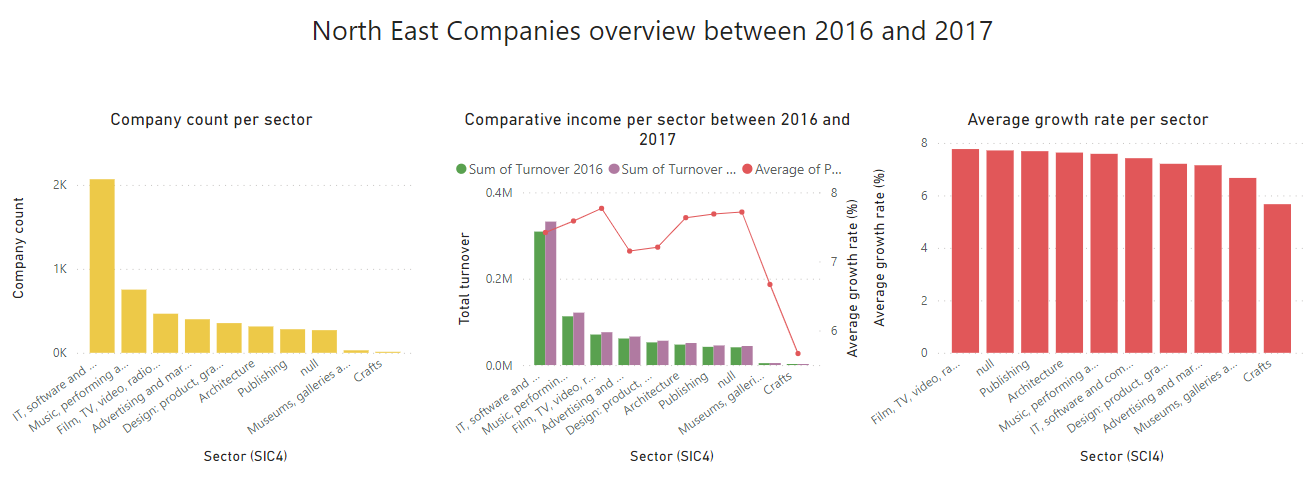
\includegraphics[width=\linewidth]{img/p2_outcome1.png}
    % \caption{Expected result for the exercise 2.3}
    % \label{fig:p2_outcome1}
\end{figure}

\subsection{Exploring companies growth}

Now that all the necessary information is displayed, enable users to explore the data by incorporating interactions such as filtering, zooming, and more.\\

Don't forget to seek feedback from a demonstrator once you have completed your work.

\end{document}